\section{Design} \label{ch4_design}
I dette afsnit dokumenteres designprocessen samt væsentlige dele af Python-koden, der anvendes til at filtrere signalet.\\
Først defineres henholdsvis filterordenen $M$, længden af filteret $l = M + 1$, en vektor $n$ med $l+1$ heltal mellem 0 og $l$ samt en vektor $x$ med $l+1$ værdier mellem $-\pi$ og $\pi$.
\\ \\
Den ideelle impulsrespons $h_d$ defineres nu som en funktion på baggrund af den ideelle amplituderespons $|H_d(\text{e}^{j\omega})|$, jf. figur \ref{fig:ideel_amp_respons}. Udledning af $h_d[n]$ findes i bilag \ref{app1}. \\
Funktionen i Python bruger vektoren $n$, ordenen $M$ samt frekvenserne $\omega_{c_1}$ og $\omega_{c_2}$ defineret ovenfor. Den ideelle impulsrespons er derfor:
\begin{align*}
h_d[n] = \begin{cases} \dfrac{\sin\left(\omega_{c_1}\left(n - \frac{M}{2}\right)\right)}{\pi\left(n - \frac{M}{2}\right)} - \dfrac{\sin\left(\omega_{c_2}\left(n - \frac{M}{2}\right)\right)}{\pi\left(n - \frac{M}{2}\right)} \quad &\text{for} \quad n \neq \frac{M}{2} \\
1 - \frac{\omega_{c_2} - \omega_{c_1}}{\pi} \quad &\text{for} \quad n = \frac{M}{2}
\end{cases}
\end{align*}
Dette er implementeret i koden således:
\begin{lstlisting}
def hd(n,M,f1,f2): 
    hd = np.zeros(len(n))
    for i in range(len(n)):
        if n[i] == M/2:
            hd[i] = 1 - (o2 - o1)/np.pi
        else:
            hd[i] = (np.sin(o1*(n[i] - M/2.)) / (np.pi*(n[i] - M/2.))) \
            - (np.sin(o2*(n[i] - M/2.)) / (np.pi*(n[i] - M/2.)))
    return hd
\end{lstlisting}
Fordi impulsresponsen er endelig skal den ideelle impulsrespons ganges med en vinduesfunktion, der herefter Fourier-transformeres for at opnå en realistisk frekvens- og amplituderespons. Der er forskellige muligheder for denne vinduesfunktion såsom det rektangulære vindue, Hamming-vinduet, Hann-vinduet og Blackman-vinduet.$^[$\footnote{Disse vinduer er beskrevet på side 559-560 i \textit{Discrete-Time Signal Processing}, Oppenheim \& Schafer (2014).}$^]$ Implementeringen af vinduerne i koden er ganske simpel, og som eksempel ses implementeringen af Hann- og Hamming-vinduet herunder:
\begin{lstlisting}
def ha(n,M,a): # Hann-vindue hvis a = 0.5. Hamming-vindue hvis a = 0.54.
    w = np.zeros(len(n))
    for i in range(len(n)):
        if n[i] >= 0 and n[i] <= M:
            w[i] = a - (1 - a)*np.cos((2*np.pi*n[i])/M)
        else:
            w[i] = 0
    return w
\end{lstlisting}

Grafen for Hamming-vinduet er vist på figur \ref{fig:Hamming}.
\begin{figure}[H]
    \centering
    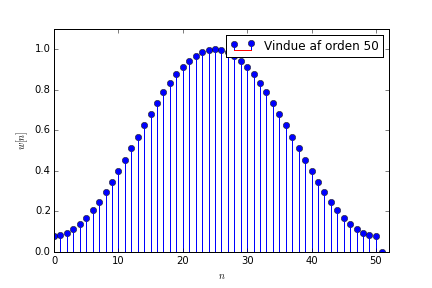
\includegraphics[width = 0.6\textwidth]{figures/Hamming-vindue.PNG}
    \caption{Eksempel på Hamming-vinduet.}
    \label{fig:Hamming}
\end{figure}

Efter implementeringen af vinduerne kaldes funktionerne for den ideelle impulsrespons og det ønskede vindue, som herefter ganges sammen. Dette resultat Fourier-transformeres ved hjælp af den implementerede FFT beskrevet tidligere. Hermed opnås frekvensresponsen $H(\text{e}^{j\omega})$ og amplituderesponsen $|H(\text{e}^{j\omega})|$, hvoraf sidstnævnte (ideelt set) er 0 mellem $\omega_{c_1}$ og $\omega_{c_2}$ og 1 ellers. Dette afhænger dog især af valget af vinduet og filterordenen $M$. Figur \ref{fig:filter_rekt} viser eksempler på anvendelsen af det rektangulære vindue for $M = 30$ og $M = 100$.

\begin{figure}[H]
\begin{minipage}{0.49\textwidth}
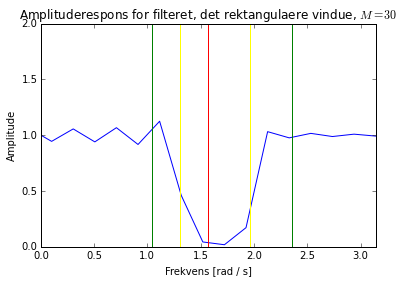
\includegraphics[width=0.9\textwidth]{figures/Filter_rekt_30.PNG}
\end{minipage}
\begin{minipage}{0.49\textwidth}
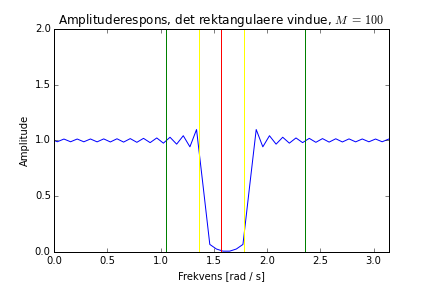
\includegraphics[width=0.9\textwidth]{figures/Filter_rekt_100.PNG}
\end{minipage}
\caption{Eksempler på båndstopfilteret under anvendelse af det rektangulære vindue og med forskellige filterordener $M$.}
\label{fig:filter_rekt}
\end{figure}

Ud fra figur \ref{fig:filter_rekt} ses det, at filteret til en vis grad overholder specifikationerne for begge værdier af $M$, at transitionsbåndet bliver smallere for højere $M$ samt at der dog er såkaldte ``ripples'' i pasbåndet. Disse ``ripples'' skyldes det rektangulære vindue, der pludselig skifter fra $0$ til $1$ og tilbage igen. For at undgå dette kan man bruge et glattere vindue som for eksempel Hamming-vinduet illustreret på figur \ref{fig:Hamming}.